\documentclass[11pt]{article}
\usepackage[UTF8]{ctex}
\usepackage[a4paper]{geometry}
\geometry{left=2.0cm,right=2.0cm,top=2.5cm,bottom=2.5cm}

\usepackage{comment}
\usepackage{booktabs}
\usepackage{graphicx}
\usepackage{diagbox}
\usepackage{amsmath,amsfonts,graphicx,amssymb,bm,amsthm}
%\usepackage{algorithm,algorithmicx}
\usepackage[ruled]{algorithm2e}
\usepackage[noend]{algpseudocode}
\usepackage{fancyhdr}
\usepackage{tikz}
\usepackage{graphicx}
\usetikzlibrary{arrows,automata}
\usepackage{hyperref}
\hypersetup{
	colorlinks=true,
	linkcolor=blue,
	filecolor=blue,      
	urlcolor=blue,
	citecolor=cyan,
}			

\setlength{\headheight}{14pt}
\setlength{\parindent}{0 in}
\setlength{\parskip}{0.5 em}

\newtheorem{theorem}{Theorem}
\newtheorem{lemma}[theorem]{Lemma}
\newtheorem{proposition}[theorem]{Proposition}
\newtheorem{claim}[theorem]{Claim}
\newtheorem{corollary}[theorem]{Corollary}
\newtheorem{definition}[theorem]{Definition}
\newtheorem*{definition*}{Definition}

\newenvironment{problem}[2][Problem]{\begin{trivlist}
\item[\hskip \labelsep {\bfseries #1}\hskip \labelsep {\bfseries #2.}]}{\hfill$\blacktriangleleft$\end{trivlist}}
\newenvironment{answer}[1][Answer]{\begin{trivlist}
\item[\hskip \labelsep {\bfseries #1.}\hskip \labelsep]}{\hfill$\lhd$\end{trivlist}}

\newcommand\E{\mathbb{E}}
\newcommand\per{\mathrm{per}}
\newcommand\eps{\varepsilon}

\title{Homework \#1}
\usetikzlibrary{positioning}

\begin{document}

\pagestyle{fancy}
\lhead{Peking University}
\chead{}
\rhead{Introduction to Theory of Computation}

\begin{center}
    {\LARGE \bf Homework \#1}\\
    {Name: Rainybunny, ID: 20120712}            % Write down your name and ID here.
\end{center}


\begin{problem}{1 (10')} ~
\begin{itemize}
    \item [(1)] (5') ~
    \begin{center}
        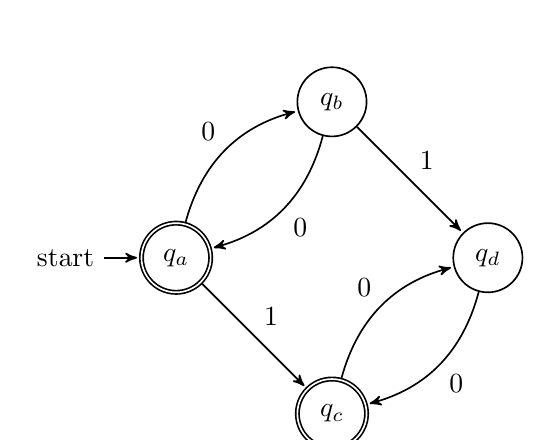
\begin{tikzpicture}[->,>=stealth',shorten >=1pt,auto,node distance=2.8cm,semithick]
            % 设置节点样式
            \tikzstyle{every state}=[fill=white,draw=black,text=black]
    
            % 定义节点
            \node[initial,state,accepting] (A) {$q_a$}; % 初始状态
            \node[state] (B) [above right of=A] {$q_b$};
            \node[state,accepting] (C) [below right of=A] {$q_c$};
            \node[state] (D) [below right of=B] {$q_d$}; % 接受状态
    
            % 定义路径
            \path
            (A) edge [bend left] node {$0$} (B)
                edge node {$1$} (C)
            (B) edge node {$1$} (D)
                edge [bend left] node {$0$} (A)
            (C) edge [bend left] node {$0$} (D)
            (D) edge [bend left] node {$0$} (C);
        \end{tikzpicture}
    \end{center}
    \item [(2)] (5') 一个三状态的 DFA 足矣.
    \begin{center}
        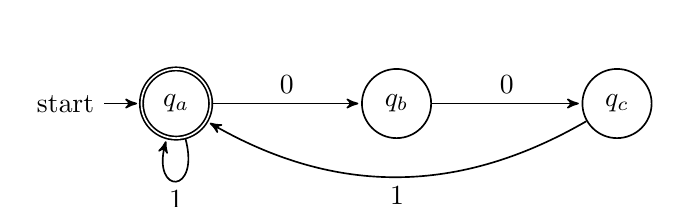
\begin{tikzpicture}[->,>=stealth',shorten >=1pt,auto,node distance=2.8cm,semithick]
            % 设置节点样式
            \tikzstyle{every state}=[fill=white,draw=black,text=black]
    
            % 定义节点
            \node[initial,state,accepting] (A) {$q_a$}; % 初始状态
            \node[state] (B) [right of=A] {$q_b$};
            \node[state] (C) [right of=B] {$q_c$};
    
            % 定义路径
            \path
            (A) edge [loop below] node {$1$} (A)
                edge node {$0$} (B)
            (B) edge node {$0$} (C)
            (C) edge [bend left] node {$1$} (A);
        \end{tikzpicture}
    \end{center}
\end{itemize}
\end{problem}

\begin{problem}{2 (20')} ~

    \qquad 设 $A$ 可由 DFA $M=(Q,\Sigma,\delta,q_0,F)$ 编码, 构造 NFA $N=(Q',\Sigma,\delta',q_0',F')$,
    其中:
    \begin{itemize}
        \item $q_0'\notin Q$, $Q'=Q\cup\{q_0'\}$, $F'=\{q_0\}$;
        \item $\delta'(q_0',\eps)=F$, 对 $q\in Q$ 和 $c\in\Sigma$, $\delta'(q,c)=\{p:\delta(p,c)=q\}$;
    \end{itemize}

    \qquad 一方面, $A^R$ 一定是 $N$ 所编码的语言 $A'$ 的子集. 对 $w=w_1\cdots w_n\in A$, 设它对应 $M$ 上的匹配路径 $q_0=r_0,r_1,\cdots,r_n$, 则 $w^R=w_n\cdots w_1$ 在 $N$ 上明显可被 $q_0',r_n,\cdots,r_1,r_0\in F'$ 接受. 另一方面, 用同理地可以说明 $(A')^R$ 是 $A$ 的子集, 这样就有 $A^R=A'$, 明所欲证.
\end{problem}

\begin{problem}{3 (20')} ~
    \begin{itemize}
        \item[(a)] (5') 有 $5$ 个. 分别是 $\{[\eps],[0],[1],[01],[11]\}$.

        \item[(b)] (5') 设 $A$ 可由 DFA $M$ 编码, 则 $A$ 将 $\Sigma^*$ 划分为不超过 $|Q|$ 个等价类. 具体地, 若 $x,y\in\Sigma^*$ 在 DFA 上匹配到同一个状态 $q$, 则根据定义, $x,y$ 等价.

        \item[(c)] (5') 设 $A$ 将 $\Sigma^*$ 划分为 $\Sigma^*=\bigsqcup_{0}^{n-1} C_i$, 不妨设 $\eps\in C_0$. 据此构造 DFA $M$, 满足
        \begin{itemize}
            \item $Q=\{q_0,\cdots,q_{n-1}\}$.
            \item $\delta(q_i,c)=q_j$, 满足 $\forall w\in C_i,~wc\in C_j$, 这是良定义的.
            \item $F=\{q_i:C_i\subset A\}$, 自然此处 $C_i$ 要么含于 $A$, 要么与 $A$ 不交.
        \end{itemize}
        显然 $M$ 编码了 $A$.

        \item[(d)] (5') $\{0^n:n\ge 0\}$ 中的字符串显然两两不等价, 等价类数量不是有限的.
    \end{itemize}
\end{problem}

\begin{problem}{4 (20')} ~

    \qquad 设 DFA $M=(Q,\Sigma,\delta,q_0,F)$ 编码 $A$, 构造 $M'=(Q,\Sigma,\delta,q_0,F')$ 满足
    $$
        F'=\{q_i:\exists w\in B,~\exists q_j\in F,~q_i\overset{w}\to q_j\}.
    $$
    其中对于 $w=w_1\cdots w_n$, $q_i\overset{w}\to q_j$ 即
    $$
        \exists q_i=p_0,p_1,\cdots,p_n=q_j\in Q,~\forall i\in[1:m],~p_i=\delta(p_{i-1},w_i).
    $$
    验证定义, 已然有 $M'$ 编码 $A/B$.
\end{problem}

\begin{problem}{5 (20')} ~
    \begin{itemize}
        \item[(a)] (10') 设该语言为 $A$. 不妨设 $\Sigma=\{0\}$, 则 $\{0^n:n\ge 0\}$ 两两不等价. 这是因为对任意 $a\neq b\in\mathbb N$, 总存在 $c$ 使得 $a+c$ 和 $b+c$ 不同时是完全平方数, 即 $0^a0^c\in A\not\Leftrightarrow 0^b0^c\in A$. 根据 \underline{Problem 3 (c)} 的结论, $A$ 不正则.
        
        \item[(b)] (10') 同理, $\{0^p:p~\text{is prime number}\}$ 两两不等价. 对任意 $0^p$ 和 $0^q$, $0^p1^p\notin A$ 然而 $0^q1^p\in A$. 所以 $A$ 不正则.
    \end{itemize}
\end{problem}

\begin{problem}{6 (10')} ~

    \qquad $A=\{2^n:n\ge 0\}$.

    \qquad 一方面, $B_2(A)=10^*$, 显然是正则的.

    \qquad 另一方面, 反证, 如果 $B_3(A)$ 满足 Pumping 引理, 对足够长的 $s$, 总存在 $x,y,z$ 使得 $s=xyz$, $|y|=\ell>0$, 且 $\forall i\ge 0,~\exists k_i\in\mathbb N,~\overline{xy^iz}=2^{k_i}$. 然而, 设 $|z|=t$,
    $$
        \begin{aligned}
            \overline{xyyz} &= \overline{xy0^\ell0^t}+\overline{yz}\\
            &= (2^{k_1}-z)3^\ell+(2^{k_1}-x3^{\ell+t})\\
            &\equiv -3^\ell(z+x3^t)\\
            &= -3^\ell\cdot 2^{k_0}\\
            &\not\equiv 0. &\pmod {2^{k_1}}
        \end{aligned}
    $$
    这与 $\overline{xyyz}=2^{k_2}$ 矛盾. 所以 $B_3(A)$ 不满足 Pumping 引理, 不正则.
\end{problem}

\end{document}